\documentclass[a4 paper]{article}
% Set target color model to RGB
\usepackage[inner=2.0cm,outer=2.0cm,top=2.5cm,bottom=2.5cm]{geometry}
\usepackage{setspace}
\usepackage{ulem}
%\usepackage[backend=biber,style=alphabetic,sorting=ynt]{biblatex}
\usepackage{natbib}
% \bibliographystyle{plainnat}
\bibliographystyle{unsrtnat}
%\usepackage[nottoc]{tocbibind}
% \addcontentsline{toc}{section}{References}
%\addbibresource{bib_Lab2.bib}
\usepackage{arydshln}
% \usepackage[rgb]{xcolor}
\usepackage[dvipsnames]{xcolor}
\colorlet{LightRubineRed}{RubineRed!70!}
\usepackage[most]{tcolorbox}
\usepackage{verbatim}
\usepackage{subcaption}
\usepackage{amsgen,amsmath,amstext,amsbsy,amsopn,tikz,amssymb,tkz-linknodes}
\usepackage{fancyhdr}
\usepackage[colorlinks=true, urlcolor=blue,  linkcolor=blue, citecolor=blue]{hyperref}
\usepackage[colorinlistoftodos]{todonotes}
\usepackage{rotating}
\usepackage{multicol}
\usepackage{graphicx}
\usepackage{listings}
\usepackage{mathtools}
%\usetikzlibrary{through,backgrounds}
\hypersetup{%
pdfauthor={Ashudeep Singh},%
pdftitle={Homework},%
pdfkeywords={Tikz,latex,bootstrap,uncertaintes},%
pdfcreator={PDFLaTeX},%
pdfproducer={PDFLaTeX},%
}
%\usetikzlibrary{shadows}
% \usepackage[francais]{babel}
\usepackage{booktabs}
\usepackage{amsmath}
\newcommand{\ra}[1]{\renewcommand{\arraystretch}{#1}}

\newtheorem{thm}{Theorem}[section]
\newtheorem{prop}[thm]{Proposition}
\newtheorem{lem}[thm]{Lemma}
\newtheorem{cor}[thm]{Corollary}
\newtheorem{defn}[thm]{Definition}
\newtheorem{rmk}[thm]{Remark}
\numberwithin{equation}{section}

\newcommand{\homework}[6]{
   \pagestyle{myheadings}
   \thispagestyle{plain}
   \newpage
   \setcounter{page}{1}
   \noindent
   \begin{center}
   \framebox{
      \vbox{\vspace{2mm}
    \hbox to 6.28in { {\bf IOC 5275:~Brain Computer Interface \hfill {\small (#2)}} }
       \vspace{6mm}
       \hbox to 6.28in { {\Large \hfill #1  \hfill} }
       \vspace{6mm}
       \hbox to 6.28in { {\it Instructor: {\rm #3} \hfill Group Number:  {\rm #5}} }% Student Id: {\rm #6}
       \hbox to 6.28in { {\it TA: #4  \hfill #6}}
      \vspace{2mm}}
   }
   \end{center}
   \markboth{#5 -- #1}{#5 -- #1}
   \vspace*{4mm}
}

\newcommand{\problem}[2]{~\\\fbox{\textbf{Problem #1}}\hfill (#2 points)\newline\newline}
\newcommand{\subproblem}[1]{~\newline\textbf{(#1)}}
\newcommand{\D}{\mathcal{D}}
\newcommand{\Hy}{\mathcal{H}}
\newcommand{\VS}{\textrm{VS}}
\newcommand{\solution}{~\newline\textbf{\textit{(Solution)}} }

\newcommand{\bbF}{\mathbb{F}}
\newcommand{\bbX}{\mathbb{X}}
\newcommand{\bI}{\mathbf{I}}
\newcommand{\bX}{\mathbf{X}}
\newcommand{\bY}{\mathbf{Y}}
\newcommand{\bepsilon}{\boldsymbol{\epsilon}}
\newcommand{\balpha}{\boldsymbol{\alpha}}
\newcommand{\bbeta}{\boldsymbol{\beta}}
\newcommand{\0}{\mathbf{0}}


\begin{document}
\homework{Lab3: Event Related Potential Analysis}{Due: 05/04/2021}{Chun-Shu Wei}{Min-Jiun Tsai}{2}{309554032, 309551176, 309540022, 0856642, 0716092, 0716085}
\noindent{\color{LightRubineRed} \rule{\linewidth}{1mm} }
\begin{center}
    \textbf{\Large{Submission Policy}}
\end{center}
\noindent{\color{LightRubineRed} \rule{\linewidth}{1mm} }
\par Read all the instructions below carefully before you start working on the assignment, and before you make a submission. For this assignment, please hand in the following your report (pdf) and code (.ipynb or .m file).
\begin{itemize}
    \item \textbf{PLAGIARISM IS STRICTLY PROHIBITED. (0 point for Plagiarism)}
    \item For mathematical problem(s), please show your work step by step and clarify statement of theorem you use (if any). Answering without mathematical derivations will get 0 point.
    \item Submission deadline: \textbf{2021.05.04 09:00:00 AM}. 
    \item \textbf{Late submission penalty formula:} $$original \ score\times(0.7)^{\#(days \ late)}$$ 
\end{itemize}
\noindent{\color{LightRubineRed} \rule{\linewidth}{0.1mm}}
\begin{center}
    \textbf{\large{File Format}}
\end{center}
\begin{itemize}
    \item Each group submits 1 report (.pdf and .tex file) and 1 code (.ipynb or .m).
    \item \textbf{Report} must contains observations, results and explanations. Please name your .pdf and .tex file as \textbf{5275\_Lab3\_GroupNum.pdf} and \textbf{5275\_Lab3\_GroupNum.tex},respectively.
    \item Paper submission is not allowed. \textbf{Please use our \LaTeX{} template to complete your report}.
    \item \textbf{Code} file must contains comments to explain your code. Please name your code file as\\ \textbf{5275\_Lab3\_GroupNum.ipynb/.m}
    \item Implementation will be graded by completeness, algorithm correctness, model description, and discussion.
    \item \textbf{Illegal format penalty:} $-5$ points for violating each rule of file format.
\end{itemize}
\noindent{\color{LightRubineRed} \rule{\linewidth}{0.1mm}}
\begin{center}
    \textbf{\large{Prerequest}}
\end{center}
To finish programming problem, you could choose Matlab or Python base on your programming preference.
\begin{multicols}{2}
\textbf{Matlab 2020a+}
\begin{itemize}
    \item \href{https://ca.nctu.edu.tw/installation/item/matlab-tah-standalone-ch}{NYCU installation page}
    \item \href{https://ca.nctu.edu.tw/manual/matlab/NCTU_MATLAB_TAH_stand_alone_installation_ch.pdf}{NCTU installation tutorial}
    \item \href{https://sccn.ucsd.edu/eeglab/downloadtoolbox.php}{EEGLab official installation page} (v2020.0+ is recommended)
\end{itemize}
\columnbreak
\textbf{Python 3.7+}
\begin{itemize}
    \item \href{https://mne.tools/stable/install/index.html}{MNE official installation page}  (0.20.7+ is recommended)
\end{itemize}
\end{multicols}
\noindent{\color{LightRubineRed} \rule{\linewidth}{0.1mm}}
\newpage
\section{Mathematical problem}
\subsection{Denoising the ERP signals--Kalman Filtering}
\subsubsection{Framework of Kalman filtering}
\begin{center}
    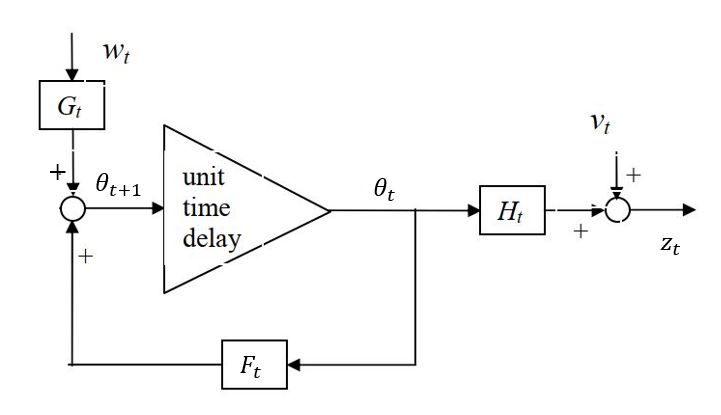
\includegraphics[height=4.5cm]{figure/state_space_representation_new.JPG}
    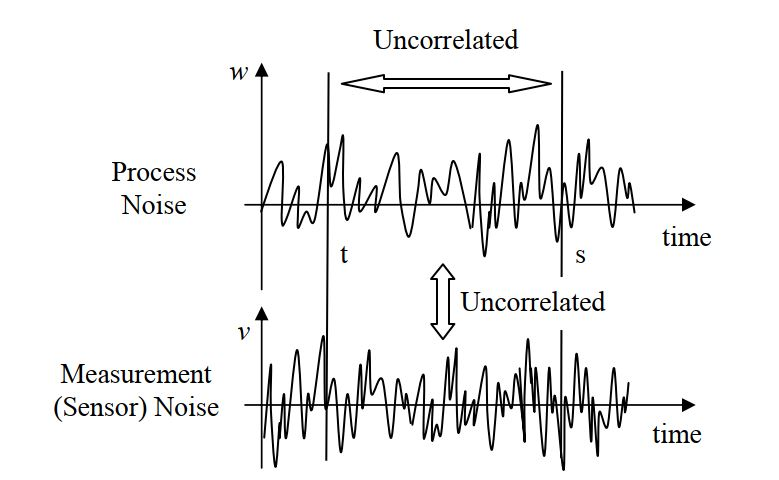
\includegraphics[height=4.5cm]{figure/noise_characteristic.JPG}
    \\\textbf{Figure: (Left) State space representation of linear time varying system (ERP) with process noise and measurement noise. (Right) Noise characteristics.}
\end{center}
\begin{tcolorbox}[colback=RoyalBlue!5!white,colframe=RoyalBlue!75!black,title=Model Formalization]
\par Let $\theta_t\in\mathbb{R}^{k\times1}$ denotes the input signal (state) and $z_t\in\mathbb{R}^{M\times1}$ denotes the output signal at time $t$. According to \textit{S. D.  Georgiadis et al.}, both $\theta_t$ and $z_t$ are defined as vector-valued processes.We could construct a state-space model for the linear dynamic systems (ERP) as below: 
\begin{equation}
    \theta_{t+1}=F_t\theta_t+G_tw_t, \ z_t=H_t\theta_t+v_t
\end{equation}
with initial condition $\theta_0$, Here we define $w_t\in\mathbb{R}^{k\times1}$ as the process noise with zero mean, $v_t\in\mathbb{R}^{M\times1}$ as the measurement noise with zero mean,  $F_t\in\mathbb{R}^{k\times k}$ as the transition matrix, and $H_t\in\mathbb{R}^{M\times k}, \ G_t\in\mathbb{R}^{k\times k}$.
\tcblower
\textbf{Hypothesis of ERP system}
\begin{itemize}
    \item $F_t$, $G_t$, and $H_t$ are known sequences of matrices
    \item $(\theta_0,w_t,v_t)$ is a sequence of mutually uncorrelated random vectors with finite variance
    \item $E[w_t]=\textbf{0}_{k\times1}, \ E[v_t]=\textbf{0}_{M\times1} \ \forall t$
    \item The covariances $C_w$, $C_v$, and $C_{wv}$ are known sequences of matrices.
\end{itemize}
Given the following conditions:
\begin{equation}
    C_v(t,s)=E[v_t\cdot v_s^T]= 
    \begin{dcases}
        \ \textbf{0}_{M\times M},& \text{where } t\neq s\\
        R_{t,M\times M},& \text{where} t=s
    \end{dcases}
\end{equation}
\begin{equation}
    C_w(t,s)=E[w_t\cdot w_s^T]= 
    \begin{dcases}
        \ \textbf{0}_{k\times k},& \text{where } t\neq s\\
        Q_{t,k\times k},& \text{where} t=s
    \end{dcases}
\end{equation}
\begin{equation}
    C_{wv}(t,s)=E[w_t\cdot v_s^T]=\textbf{0}_{k\times M}, \ \forall t, \ \forall s
\end{equation}
\end{tcolorbox}
To obtain an optimal value of $\theta_t$ based on measurements $z_t$, we minimize the mean square error:
\begin{equation}
    J_t=E[(\hat{\theta}_t-\theta_t)^T(\hat{\theta}_t-\theta_t)]
\end{equation}
with the constraints (1.1) to (1.4).
We call $\hat{\theta}_{t|t-1}$ as expected state transition based on model, $\hat{z}_t$ as expected output.
\begin{equation}
    \begin{split}
        &\theta_t=F_{t-1}\theta_{t-1}+G_{t-1}w_{t-1}\\
        &\hat{\theta}_{t|t-1}=E[F_{t-1}\hat{\theta}_{t-1}+G_{t-1}w_{t-1}]=F_{t-1}\hat{\theta}_{t-1}+G_{t-1}E[w_{t-1}]\\
        &\hat{z_t}=E[H_t\hat{\theta}_{t|t-1}+v_t]=H_t\hat{\theta}_{t|t-1}+E[v_t]=H_{t}\hat{\theta}_{t|t-1}
    \end{split}
\end{equation}
\begin{center}
    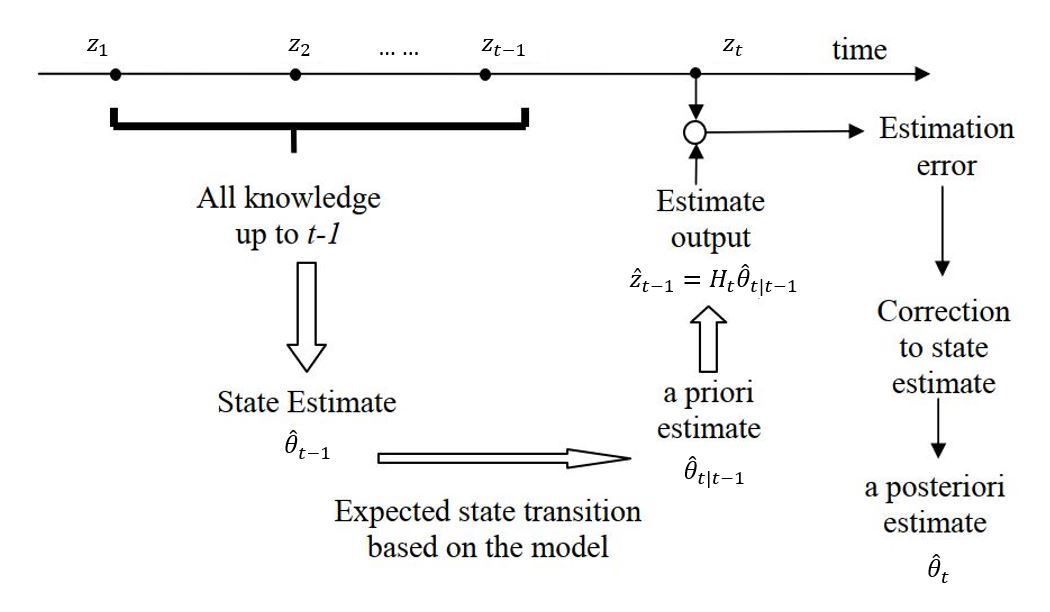
\includegraphics[height=7cm]{figure/kalman_filter_flowchart_new.JPG}\\
    \textbf{Figure: Outline of the Kalman filter algorithm}
\end{center}
\subsubsection{Correction of the state estimate} 
\par Assimilating the new measurement $z_t$, we can update the state estimate in proportion to the output estimation error.
\begin{equation}
    \hat{\theta}_t=\hat{\theta}_{t|t-1}+K_{t}(z_t-\hat{z}_t)
\end{equation}
Let $\epsilon_t=\hat{\theta}_{t|t-1}-\theta_t$ be a priori estimation error, then
\begin{equation}
\begin{split}
    e_t&\equiv\hat{\theta}_t-\theta_t=\hat{\theta}_{t|t-1}+K_t\big(z_t-H_t\hat{\theta}_{t|t-1}\big)-\theta_t\\
    &=\hat{\theta}_{t|t-1}+K_t\big(H_{t}\theta_t+v_t-H_t\hat{\theta}_{t|t-1}\big)-\theta_t=\big(\hat{\theta}_{t|t-1}-\theta_t\big)-K_{t}H_t\big(\hat{\theta}_{t|t-1}-\theta_t\big)+K_{t}v_t\\
    &=\big(I_k-K_tH_t\big)\epsilon_t+K_tv_t
\end{split}
\end{equation}
Equation (1.7) provides a structure of linear filter in recursive form. Denoting $K_t\in\mathbb{R}^{k\times M}$ as a gain 
matrix to be optimized so that the mean squared error (expectation of $e_t^Te_t$) of state estimation may be minimized.

\begin{tcolorbox}[colback=RubineRed!5!white,colframe=RubineRed!75!black]
    \problem{1}{5}
    Please show that 
    \begin{equation}
        e_t^Te_t=\epsilon_t^T\epsilon_t+\epsilon_t^TH_t^TK_t^TK_tH_t\epsilon_t-2\epsilon_t^TK_tH_t\epsilon_t+2\epsilon_t^TK_t^Tv_t-2v_t^TK_t^TK_tH_t\epsilon_t+v_t^TK_t^TK_tv_t
    \end{equation}
\end{tcolorbox}
\begin{tcolorbox}[colback=YellowGreen!5!white,colframe=YellowGreen!75!black,title={Problem 1's answer}]
    First, we calculate and rewrite $e_t$ and $e_t^T$\newline
    $e_t=(I_k-K_tH_t)\epsilon_t+K_tv_t=\epsilon_t-K_tH_t\epsilon_t+K_tv_t$ \newline
    $e_t^T=\epsilon_t^T(I_k-K_tH_t)^T+v_t^TK_t^T=\epsilon_t^T(I_k-H_t^TK_t^T)+v_t^TK_t^T=\epsilon_t^T-\epsilon_t^TH_t^TK_t^T+v_t^TK_t^T$\newline
    \newline
    $e_t^Te_t=\epsilon_t^T\epsilon_t-\epsilon_t^TK_tH_t\epsilon_t+\epsilon_t^TK_tv_t-\epsilon_t^TH_t^TK_t^T\epsilon_t+\epsilon_t^TH_t^TK_t^TK_tH_t\epsilon_t$\newline
    \hspace*{0.5cm}$-\epsilon_t^TH_t^TK_t^TK_tv_t+v_t^TK_t^T\epsilon_t-v_t^TK_t^TK_tH_t\epsilon_t+v_t^TK_t^TK_tv_t$\hspace*{0.2cm}\textcolor{red}{--\ eq(1)}\newline
    \newline
    We know that $\left(\epsilon_t^TK_tH_t\epsilon_t\right)^T=\epsilon_t^TH_t^TK_t^T\epsilon_t$ and $\left(\epsilon_t^TK_tv_t\right)^T=v_t^TK_t^T\epsilon_t$\newline
    \hspace*{0.5cm}and $\left(v_t^TK_t^TK_tH_t\epsilon_t\right)^T=\epsilon_t^TH_t^TK_t^TK_tv_t$ and all of them are const\newline
    \newline
    Hence, we can rewrite \textcolor{red}{eq(1)} to \newline
    $e_t^Te_t=\epsilon_t^T\epsilon_t+\epsilon_t^TH_t^TK_t^TK_tH_t\epsilon_t-2\epsilon_t^TK_tH_t\epsilon_t+2\epsilon_t^TK_tv_t-2v_t^TK_t^TK_tH_t\epsilon_t+v_t^TK_t^TK_tv_t$
\end{tcolorbox}
Let us differentiate the scalar function $e_t^Te_t$ with respect to matrix $K_t$ by using the following matrix differentiation rules.
\begin{tcolorbox}[colback=RoyalBlue!5!white,colframe=RoyalBlue!75!black]%neRed!75!black
\textbf{Matrix differentiation rule 1}\\
Let $a\in\mathbb{R}^{k\times1}$, $b\in\mathbb{R}^{M\times1}$, and $K\in\mathbb{R}^{k\times M}$ is same as above $K_t$ (We omit the subscript $t$ for brevity).
    \begin{align}
        f\equiv[a_1,...,a_k]\begin{bmatrix}
        K_{11}& \dots & K_{1M}\\
        \vdots& \ddots & \vdots\\
        K_{k1}& \dots & K_{kM}\
        \end{bmatrix}\begin{bmatrix}
        b_1\\\vdots\\b_M
        \end{bmatrix}=a^TKb\Rightarrow\frac{df}{dK}=\Big[\frac{\partial f}{\partial K_{ij}}\Big]=[a_ib_j]=ab^T, \ \forall i\in\mathbb{Z}_{k}, j\in\mathbb{Z}_{M}
    \end{align}
\tcblower
\textbf{Matrix differentiation rule 2}\\
Let $ b,c\in\mathbb{R}^{M\times1}$, and $ K\in\mathbb{R}^{k\times M}$, and $g=c^TK^TKb$, then
\begin{equation}
    \frac{dg}{dK_t}=\Big[\frac{\partial g}{\partial K_{im}}\sum_{i=1}^M\sum_{j=1}^k\sum_{l=1}^k K_{il}c_lK_{ij}b_j\Big]=\Big[\sum_{j=1}^k c_mK_{ij}b_j+\sum_{j=1}^k K_{il}c_lb_m\Big]=Kbc^T+Kcb^T
\end{equation}
\end{tcolorbox}
\begin{tcolorbox}[colback=RubineRed!5!white,colframe=RubineRed!75!black]
\problem{2}{15}
Use the matrix differentiation rule 1 and 2 to show that
\begin{equation}
    \frac{de_t^Te_t}{dK_t}=2K_tH_t\epsilon_t\epsilon_t^TH_t^T -2[K_tH_t\epsilon_{t}v_t^T + K_tv_t\epsilon_t^TH^T_t ] + 2K_tv_tv_t^T + 2[\epsilon_tv^T_t- \epsilon_t\epsilon_t^TH^T_t ]
\end{equation}
\end{tcolorbox}
The necessary condition for the mean squared error of state estimate with respect to the gain matrix $K_t$ is:
$$\frac{dJ_t}{dK}=\textbf{0}_{k\times M}$$
Taking expectation of $e_t^Te_t$ , differentiating it w.r.t. $K_t$ and setting it to zero yield:
\begin{equation}
    E[K_tH_t\epsilon_t\epsilon_t^TH_t^T -K_tH_t\epsilon_{t}v_t^T - K_tv_t\epsilon_t^TH^T_t + K_tv_tv_t^T + \epsilon_tv^T_t- \epsilon_t\epsilon_t^TH^T_t]=\textbf{0}_{k\times M}
\end{equation}
Which means that $K_t$ and $H_t$ can be factored out, 
\begin{equation}
    K_tH_tE[\epsilon_t\epsilon_t^T]H^T_t-K_tH_tE[\epsilon_tv^T_t ] - K_tE [ v_t\epsilon_t^T]H^T_t + K_tE[ v_tv^T_t ] + E[\epsilon_tv^T_t]-E[\epsilon_t\epsilon_t^T ]H^T_t = \textbf{0}_{k\times M}
\end{equation}
Since we know that 
\begin{equation}
    \hat{\theta}_{t|t-1} = E[F_{t-1}\hat{\theta}_{t-1}+ G_{t-1}w_{t -1}]=F_{t-1}\hat{\theta}_{t-1}
\end{equation}
and $$\epsilon_t=\hat{\theta}_{t|t-1}-\theta_t,$$
we can examine $E[\epsilon_tv_t^T]=E[(\hat{\theta}_{t|t-1}-\theta_t)v_t^T]=E[(\hat{\theta}_{t|t-1}v_t^T]-E[\theta_tv_t^T]=\textbf{0}_{k\times M}$
\begin{tcolorbox}[colback=RubineRed!5!white,colframe=RubineRed!75!black]
\problem{3}{10}
Please show that 
\begin{equation}
    E[\epsilon_tv_t^T]=\textbf{0}_{k\times M} \ \& \ E[v_t\epsilon_t^T]=\textbf{0}_{M\times k}
\end{equation}
\end{tcolorbox}
Let us define the error covariance of a priori state estimation
\begin{equation}
    C_{\hat{\theta}_{t|t-1}}\equiv E[\epsilon_t\epsilon_t^T]=E[(\hat{\theta}_{t|t-1}-\theta_t)(\hat{\theta}_{t|t-1}-\theta_t)^T]
\end{equation}
\begin{tcolorbox}[colback=RubineRed!5!white,colframe=RubineRed!75!black]
\problem{4}{5}
Please show that 
\begin{equation}
    K_t=C_{\hat{\theta}_{t|t-1}}H_t^T\Big(H_tC_{\hat{\theta}_{t|t-1}}H_t^T+C_v(t,t)\Big)^{-1}
\end{equation}
Such $K_t$ is called the \textbf{Kalman Gain}. 
\end{tcolorbox}
\subsubsection{Updating the Error Covariance } 
% 還要補說明
The above Kalman gain contains the a priori error covariance $C_{\hat{\theta}_{t|t-1}}$ . This must be updated recursively based on each new measurement and the state transition model. 
Define the a posteriori state estimation error covariance
\begin{equation}
    C_{\hat{\theta}_{t}}=E[e_{t}e_t^T]=E[(\hat{\theta}_{t}-\theta_t)(\hat{\theta}_{t}-\theta_t)^T]
\end{equation}
\begin{tcolorbox}[colback=RubineRed!5!white,colframe=RubineRed!75!black]
\problem{5}{5}
Please show that 
\begin{equation}
    C_{\hat{\theta}_{t}}=(I_k-K_tH_t)C_{\hat{\theta}_{t|t-1}}
\end{equation}
\end{tcolorbox}
Derive (1.21), one cancan compute $C_{\hat{\theta}_{t+1|t}}$ by using the state transition equation (1.1).\\
Consider
\begin{equation}
\epsilon_{t+1}=\hat{\theta}_{t+1|t}-\theta_{t+1|t}=F_t\hat{\theta}_t-(F_t\theta_t+G_t{w}_t)=F_{t}e_t-G_{t}w_t.
\end{equation}
From (1.17)
\begin{equation}
\begin{split}
    C_{\hat{\theta}_{t+1|t}}&=E[\epsilon_{t+1}\epsilon_{t+1}^T]\\
    &=E[(F_{t}\theta_t+G_tw_t)(F_{t}\theta_t+G_tw_t)^T]\\
    &=F_tE[e_te_t^T]F_t^T-G_tE[w_te_t^T]F_t^T-F_tE[e_tw_t^T]G_t^T+G_tE[w_tw_t^T]G_t^T
\end{split}
\end{equation}
\begin{tcolorbox}[colback=RubineRed!5!white,colframe=RubineRed!75!black]
\problem{6}{5}
Please show that 
\begin{equation}
     C_{\hat{\theta}_{t|t-1}}=F_{t-1} C_{\hat{\theta}_{t-1}}F_{t-1}^T+G_{t-1}C_{w}(t-1,t-1)G_{t-1}^T
\end{equation}
\end{tcolorbox}
\subsubsection{The Recursive Calculation Procedure for the Discrete Kalman Filter}
\begin{center}
    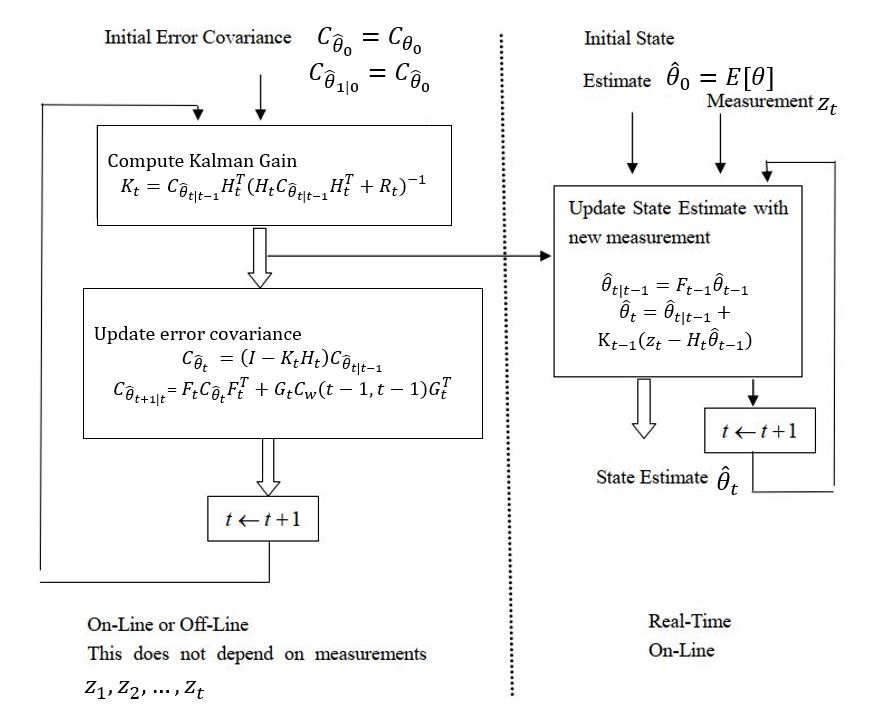
\includegraphics[height=14cm]{figure/recursive_new.JPG}\\
    \textbf{Figure: Solve discrete Kalman Filter recursively}
\end{center}
\newpage
\section{Multiple choices}
Please give a brief explanation for option(s) you choose. Answering without any description will get 0 point.
\begin{tcolorbox}[colback=RubineRed!5!white,colframe=RubineRed!75!black]
\problem{7}{5}%6.7
Which of the following statements are true regarding baseline correction? Assume that we are using \textbf{stimulus-locked epochs}.
\begin{itemize}
    \item[(A)]To perform baseline correction, the mean voltage is calculated during the prestimulus portion of the epoch, and this value is then subtracted from every point in the prestimulus period.
    \item[(B)]To perform baseline correction, the mean voltage is calculated during the prestimulus portion of the epoch, and this value is then subtracted from every point in the waveform.
    \item[(C)]We take the mean of the prestimulus period (rather than just taking the voltage at time zero) so that we can average out random noise during the prestimulus period and obtain a better estimate of the voltage offset.
    \item[(D)]We take the mean of the prestimulus period (rather than just taking the voltage at time zero) so that we can obtain a better estimate of the noise level.
\end{itemize}
\end{tcolorbox}
\begin{tcolorbox}[colback=RubineRed!5!white,colframe=RubineRed!75!black]
\problem{8: Single choice}{5} 
Imagine that a researcher conducts a study comparing a patient group with a control group in an oddball paradigm. The researcher conducts a separate patient/control $x$ rare/frequent ANOVA for each time point from 0-800 ms at each electrode site. Each ANOVA yielded 3 $p$ values (main effect of patient/control, main effect of rare/frequent, and interaction). The sampling rate was 250 Hz, so there were 200 time points between 0 and 800 ms. There were 32 electrode sites. If there are no true differences between groups, how many significant p values would you expect the researcher to obtain as a result of noise in the data? [For simplicity, assume that every time point and electrode site is independent of every other time point and electrode site. Assume that $\alpha=0.05$.]\\
(A) 1280 (B) 507 (C) 320 (D) 960
\end{tcolorbox}
\begin{tcolorbox}[colback=RubineRed!5!white,colframe=RubineRed!75!black]
\problem{9}{5}%8.5
Imagine that a researcher conducts a go/no-go experiment in which subjects are supposed to press a button every time they see the word GO (written in green, 80\% of trials) and to make no response when they see the word STOP (written in red, 20\% of trials). And imagine that they find a larger N1 wave (at 170 ms) for the STOP stimulus than for the GO stimulus. Could this effect be plausibly explained by a physical stimulus confound? 
\begin{itemize}
    \item[(A)]No. It is unlikely that the small physical differences between GO and STOP could explain a difference at 170 ms.
    \item[(B)]Yes, because subjects may have been looking at a different places on the screen when the words GO and STOP appeared, which would change the position of the stimulus on the retina.
    \item[(C)]Yes, because the word STOP contains more letters than the word GO and therefore might elicit a larger N1.
    \item[(D)] Yes, because it is possible that red stimuli elicit a larger N1 than green stimuli.
\end{itemize}
\end{tcolorbox}
\begin{tcolorbox}[colback=RubineRed!5!white,colframe=RubineRed!75!black]
\problem{10}{5}
The time-frequency plot below shows data from the oddballs in a mismatch negativity paradigm. Which of the following statements are true about this plot? 
\begin{multicols*}{2}
\begin{center}
    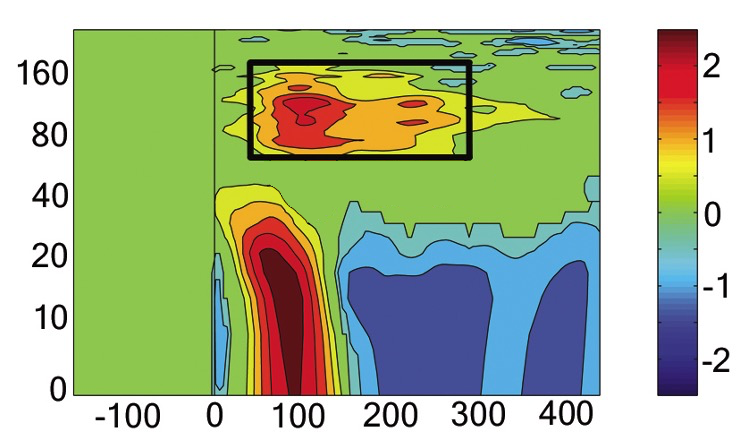
\includegraphics[height=4.5cm]{figure/Time-Frequency.png}
\end{center}
\columnbreak
\begin{itemize}
    \item[(A)] The X axis is time.
    \item[(B)] The Y axis is a measure of magnitude (typically amplitude or power).
    \item[(C)] If we wanted to reproduce the original data from a set of wavelets, we would need some high-amplitude wavelets centered at ~100 ms with frequencies ranging from 0 to ~20 Hz (in addition to wavelets at other frequencies).
    \item[(D)] The activity shown in the box from ~80-280 milliseconds is probably a genuine oscillation.
\end{itemize}
\end{multicols*}
\end{tcolorbox}
\section{Coding problem}
\begin{tcolorbox}[colback=RubineRed!5!white,colframe=RubineRed!75!black]
\problem{11: Auditory Oddball paradigm}{2+2+2+2+2+2+2=16}
Please use the data: Day1 \_ERP.set to answer these questions.\\
\textbf{Data Information}\\
This data contains 2 sessions, been down-sampled to $250Hz$, and been band-pass filtered.
\begin{center}
   \begin{tabular}{||c|c||}
    \hline
    Trigger & Event\\
    \hline
     10 & Response \\
     2 & High pitch\\
     3 & Low pitch\\
     4 & End of session\\
     \hline
    \end{tabular}
\end{center}
\subproblem{a} Please guess the range of band-pass filtered and show how you find this range.
\subproblem{b} Please guess the portion of High Pitch: Low pitch and show how you find it. 
\subproblem{c} Plot the Fz, Cz, and Pz's average ERP for Response respectively.
\subproblem{d} Plot the Fz, Cz, and Pz's average ERP for High pitch and Low pitch respectively.\\
\tcblower
\textbf{For subproblem (e) and (f), please plot topolots for P300.}\\
Suppose that for each channel, P300 occurs during $[300,400]msec$ when $t=0$ indicates onset time of High pitch and Low pitch. That is, $P300^{ch}\in\mathbb{R}^{51\times1} \ \forall ch\in\mathbb{Z}_{30}$.
\subproblem{e} Plot topoplot for High pitch and Low pitch respectively. (Use $mean(P300^{ch}) \ \forall ch\in\mathbb{Z}_{30}$) \\
$\forall ch\in\mathbb{Z}_{30}$, define Min-Max normalization as below
\begin{equation}
    \frac{mean(P300^{ch})-\min{\big\{mean(P300^{ch})\big|ch\in\mathbb{Z}_{30}\big\}}}{\max{\big\{mean(P300^{ch})\big|ch\in\mathbb{Z}_{30}\big\}}-\min{\big\{mean(P300^{ch})\big|ch\in\mathbb{Z}_{30}\big\}}}
\end{equation}
\subproblem{f} Plot topoplot for High pitch and Low pitch respectively with Min-Max normalization.
\\If we define signal-to-noise ratio (SNR) for each channel as below:
\begin{equation}
    SNR^{ch}=
    \frac{P300^{ch}}{std{(Baseline^{ch})}}
\end{equation}
where baseline interval $[-200, 0]msec$, $Baseline^{ch}$ is mean by trial, and $t=0$ indicates onset time of High pitch and Low pitch. 
\subproblem{g} For each channel, plot SNR for High picth and Low pitch. (Bar plot)
\subproblem{h} Plot cumulative (by trial) SNR for  Fz, Cz, and Pz channel and give a description of your observation.
\end{tcolorbox}

\begin{tcolorbox}[colback=RubineRed!5!white,colframe=RubineRed!75!black]
\problem{12: 5 target SSVEP paradigm}{4+8+7=19}
Please use the data: Day 2\_SSVEP.set to answer these questions.
\\\textbf{Data Information}
\begin{center}
   \begin{tabular}{||c|c||}
    \hline
    Trigger & Event\\
    \hline
     11 & 10 $Hz$ \\
     21 & 11 $Hz$\\
     31 & 12 $Hz$\\
     41 & 13 $Hz$\\
     51 & Nan\\
     \hline
    \end{tabular}
\end{center}
\subproblem{a} For Fz and Oz, please plot average ERP for each type of stimuli.
\\\textbf{Apply short time Fourier transform (\href{https://www.mathworks.com/help/signal/ref/spectrogram.html}{spectrogram in matlab}) with the following parameters to answer subproblem (b).} 
\begin{lstlisting}[language=Matlab]
% B: SSVEP for certain channel, sfreq:sampling rate
% P is a power spectrum density matrix with size (N_freq, N_time)
[S,F,T,P]=spectrogram(B,sfreq,sfreq/2,sfreq,sfreq);
\end{lstlisting}
\subproblem{b} Plot power v.s. frequency for each stimuli at $F_z$ and $O_z$ channel and give description of your observation.
\\\textbf{We extract $\{10,11,12,13\}Hz$ from PSD you get from subproblem (b), and called it as response frequency.}
\subproblem{c} Plot topolot of response $Hz$ v.s. stimuli $Hz$ with same Min-Max normalization technique. That is, you will plot $4\times5=20$ topoplots this time.
\end{tcolorbox}

\begin{thebibliography}{6}
\bibitem{Kalman Filter}
Stefanos D. Georgiadis, Perttu O. Ranta-aho, Mika P. Tarvainen, Pasi A. Karjalainen, 
\textit{Single-Trial Dynamical Estimation of Event-Related Potentials: A Kalman Filter-Based Approach}, IEEE Transactions on Biomedical Engineering, 52(8), 2005.
\bibitem{Lecture Note}
Harry Asada, Lecture notes for \textit{Identification, Estimation, and Learning}, Massachusetts Institute of Technology, 
 Department of Mechanical Engineering, 2006.
\bibitem{EEG Signal Processing}
S. Sanei, J.A. Chambers, \textit{EEG Signal Processing}, Wiley, 2007. \bibitem{YPL Lecture note}
Yuan-Pin Lin, Lecture notes for \textit{$3^{rd}$ EEG summer workshop}, National Sun Yat-sen University, Institute of Medical Science and Technology, 2020.
\bibitem{Cohen} 
Mike X Cohen. \textit{Analyzing neural time series data : theory and practice.} Cambridge, Massachusetts :The MIT Press, 2014.

%Knuth: Computers and Typesetting,
%\\\texttt{http://www-cs-faculty.stanford.edu/\~{}uno/abcde.html}

\bibitem{EEG_principal}
Donald L. Schomer and Fernando H. Lopes da Silva,
\textit{Niedermeyer's Electroencephalography: Basic Principles, Clinical Applications, and Related Fields},Lippincott William \& Wilkins, 2011. \textbf{ISBN} 9780781789424.

\end{thebibliography}
\newpage
\section{Feedback for Lab 3}
This part is not for grading but for understanding learning situation of each student. Please give us your feedback and comments.
\subsection{Work Division}
For example,\\
\begin{center}
    \begin{tabular}{||c|c|c||}
    \hline
     Student ID & Name & Be response for... ... \\
    \hline
     123456789 & Tony & solving Problem 1 and designing preprocessing algorithm in problem 7\\
     \hline
     987654321 & May & solving Problem 3 and designing preprocessing algorithm in problem 7\\
     \hline
      & & \\
     \hline
\end{tabular}
\end{center}
\subsection{Suggestions and Comments}
\subsubsection{For instructor}
\subsubsection{For teaching assistant(s)}
\textbf{4.2.2.a For Min-Jiun}\\
\textbf{4.2.2.b For Eric}\\
\noindent{\color{LightRubineRed} \rule{\linewidth}{0.5mm}}
\begin{center}
    \large{\textbf{Office Hour Information}}
\end{center}
\par We'll have limited time to teach EEGLab and MNE on our course; therefore, if you have any question about lab 2, feel free to make an appointment or come to ask me during my office hour.\\
\begin{center}
    \begin{tabular}{||c|c|c||}
    \hline
    Day & Time & Office\\
        \hline\hline
          Tue. & 12:20 p.m.-13:10 p.m. & EC120 \\
          \hline
          Thur. & 06:30 p.m.-09:30 p.m. & SC207\\
          \hline
    \end{tabular}
\end{center}
\textbf{Note}\\
Actually, my office hour on Thursdays is main for calculus consultation. If there are undergraduate students come to ask calculus problems, I need to teach them first and then to solve your problem during the rest of the office hour on Thursday nights.\\
\noindent{\color{LightRubineRed} \rule{\linewidth}{0.5mm}}
\end{document} 